\documentclass[12pt,a4paper,twoside]{report}
\usepackage[left=2cm,right=2cm,top=1.5cm,bottom=1.5cm]{geometry}
\usepackage{titlesec}
\titleformat{\chapter}[display]   
{\normalfont\huge\bfseries}{\chaptertitlename\ \thechapter}{20pt}{\Huge}   
\titlespacing*{\chapter}{0pt}{-55pt}{40pt}
\titlespacing*{\section}{0pt}{\baselineskip}{\baselineskip}
\vspace{-\baselineskip}
\usepackage{pagenote}
\usepackage{algorithm}
\usepackage{algorithmic}
\usepackage{graphicx}
\usepackage[utf8]{inputenc}	% Para caracteres en español
\usepackage{amsmath,amsthm,amsfonts,amssymb,amscd}
\usepackage{multirow,booktabs}
\usepackage[table]{xcolor}
\usepackage{fullpage}
\usepackage{lastpage}
\usepackage{enumitem}
\usepackage{fancyhdr}
\usepackage{mathrsfs}
\usepackage{wrapfig}
\usepackage{setspace}
\usepackage{calc}
\usepackage{color,soul}
\usepackage{multicol}
\usepackage{cancel}
\usepackage[retainorgcmds]{IEEEtrantools}
\usepackage{xcolor}
\colorlet{shadecolor}{orange!15}
\parindent 0in
\parskip 12pt
\geometry{margin=1in, headsep=0.25in}
\theoremstyle{definition}
\newtheorem{defn}{Definition}
\newtheorem{reg}{Rule}
\newtheorem{exer}{Exercise}
\newtheorem{note}{Note}
\usepackage{listings}
\usepackage{spverbatim}
\usepackage{fancyvrb}
\usepackage{hyperref}
\usepackage{float} 
\usepackage{natbib}
\usepackage{tikz}
\usepackage{pgfplots}
\usepackage{pgfplotstable}
\usepackage{soulutf8}
\usepackage{color,soul}
\usepackage{xcolor}
\usepackage{tabularx}
\newtheorem{lemma}{Lemma}[section]
\newtheorem{theorem}{Theorem}[section]
\newtheorem{proposition}{Proposition}[section]
\newtheorem{definition}{Definition}[section]
\DeclareMathOperator*{\argmax}{argmax}
\newcommand{\domain}[1]{\texttt{\textsc{#1}}}
\newcommand\minus{\mathop{\mbox{$\mathit{.e}$-}}}
\usepackage[draft]{todo}
\usepackage{mathtools,xparse}
\DeclarePairedDelimiter{\abs}{\lvert}{\rvert}
\DeclarePairedDelimiter{\norm}{\lVert}{\rVert}
\NewDocumentCommand{\normL}{ s O{} m }{%
  \IfBooleanTF{#1}{\norm*{#3}}{\norm[#2]{#3}}_{L_1(\Omega)}%
}
\newcommand{\fyTodo}[1]{\Todo[FY:]{\textcolor{orange}{#1}}}
\newcommand{\fyTodostar}[1]{\Todo*[FY:]{\textcolor{orange}{#1}}}
\newcommand{\fyDone}[1]{\done[FY]\Todo[FY:]{\textcolor{orange}{#1}}}
\newcommand{\fyDonestar}[1]{\done[FY]\Todo[FY:]{\textcolor{orange}{#1}}}
\pgfkeys{
    /tr/rowfilter/.style 2 args={
        /pgfplots/x filter/.append code={
            \edef\arga{\thisrow{#1}}
            \edef\argb{#2}
            \ifx\arga\argb
            \else
                \def\pgfmathresult{}
            \fi
        }
    }
}

\begin{document}
\setlength{\belowdisplayskip}{8pt} \setlength{\belowdisplayshortskip}{8pt}
\setlength{\abovedisplayskip}{8pt} \setlength{\abovedisplayshortskip}{8pt}
\setlist{nosep}
\setlength{\parskip}{0.1cm}
\setlength{\parindent}{1em}
\section*{Introduction}
Neural Machine Translation (will be referred to as NMT in the rest of the article) has achieved the state of the art performance in Automatic Translation since 2015 and became the main architecture in industrial development and natural language processing research. Neural Machine Translation’s quality is assured both theoretically and empirically under the assumption of the matching between training data distribution and testing data distribution. However, this situation is hardly true in real contexts where the NMT model is often trained with big training data which is heterogeneous in terms of topic and size of the size of topics data, and one needs to make the best to robustly handle inputs from unexpected domains in the testing phase.
\subsection*{Overview}
Data-based Machine Translation whether statistical or neural is based on well-studied machine learning principles. Given a training set, $\mathbf{S_{trn}}$ drawn from a distribution $\mathbf{D_s}$ consisting of sentence pairs $(f,e)$, the parameter of the probabilistic model $P_{\theta}$ is optimized by minimizing empirical expectation of a loss function
$$l(h_{\theta}(f,e)) = \frac{1}{N}\displaystyle{\mathop{\sum_{(f,e)\in \mathbf{S_{trn}}}l(h_{\theta}(f,e))}}$$
Then in the testing phase, given an example drawn from the same underlying distribution $\mathbf{D_s}$, the accuracy of the trained model is assured by a statistical upper bound composed of 2 terms as empirical training loss and the capacity of hypothesis space $h_{\theta}$ divided by a factor of training set size. However, if testing samples are drawn from a different source, the upper bound can no longer be applied.

In this thesis, we are interested in several problems arising in multi-domain contexts
\begin{itemize}
	\item Multi-domain Adaptation.
		\begin{itemize}
			\item with labeled data.
			\item with unlabeled data (unsupervised adaptation).
		\end{itemize}
	\item Robustness to out of domain data.
\end{itemize}

The first problem was first studied under the concept of Domain Adaptation where one aims to improve the poor performance of the model trained in a low resource domain by leveraging different high resource domains. In general, the methods for Domain Adaptation problem can be categorized into 2 classes: data-based methods and model-based methods.

\subsection*{State of the art}

\subsubsection*{Data-based adaptation methods}
Methods in this category improve the low resource model by collecting domain-related examples from out-of-domain resources. For the statistical model, \cite{mansour12simple} investigated the use of the Moore-Lewis score to re-estimate the phrase table.\cite{Duh13selection,Axelrod11domain,silva2018extracting} proposed several methods to select examples for training NMT model by scoring based on the cosine similarity of distributed sentence embedding or based on the probability calculated by in-domain Neural Language Model and the cosine similarity of $tf\_idf$ embedding adjusted by Feature decay algorithm. Another way to get more training is to create pseudo parallel data, \cite{Junjie19domain} proposed an unsupervised method to create pseudo in-domain training data using word by word translation.

\subsubsection*{Model-based adaptation methods}
These approaches take interest in the model architecture and model training process. We can further categorize them into 3 classes: feature-augmentation, module-augmentation, surrogate losses, and finetuning. In the class of feature-augmentation, \cite{Kobus17domain}, \cite{kenji17multi}, \cite{Pham19generic} proposed to add domain-tags and learn-able domain-embeddings to existing word feature of NMT model. These methods are cheap and efficient in terms of gain over model-size.


Module-augmentation is more expensive then feature-augmentation because one adds one or several complementary layers into standard NMT architecture; \cite{bapna19simple},\cite{Michel18extreme},\cite{Zheng18multi},\cite{Vilar18learning}, \cite{Britz2017mixing} are included in this category. Residual module in \cite{bapna19simple} and Hidden units in \cite{Vilar18learning} (\ref{fig:overview}) are used as a plug-in which is used to fine-tune the model without
changing the value of the main model. \cite{Zheng18multi} (\ref{fig:overview}) added 2 gates to extract domain agnostic representations and domain-specific representations from the output of encoder which are then plugged to the decoder. \cite{Britz2017mixing} (\ref{fig:overview}) also plugged a domain-classifier on top of the encoder to force the domain-specific representation. \cite{domhan2017using} added a Language Model-like module between target embedding and the decoder so that the decoder can benefit from the monolingual data of the target domain in the target language. The architecture is shown in figure (\ref{fig:overview}). \cite{dakwle17fine} (\ref{fig:overview}) proposed a multi-output layer for domain-model which are trained by minimizing the cross-entropy for in-domain examples and Kullback-Leibler distance to
the conditional distribution of a teacher generic model. The proposed model has 2 output layers, each of them optimizing one of 2 losses respectively. \cite{Dou19Unsupervised} attempted to use only monolingual target data for adapting to a new domain by using additional learnable domain embedding and task embedding and introducing language modeling tasks in the target language. 


In machine learning theory and practice, surrogate losses are used to stabilize the training and to improve model generalization. In Domain Adaptation NMT, for example, \cite{Chen17cost} used domain-classification loss in addition to cross-entropy loss to leverage out of domain data while adapting to the target domain. 


The last is fine-tuning category according to which models are pretrained with out-of-domain data, then continue being trained with in-domain data during a few training epochs. \cite{Thomas11limsi}  proposed this practice to adapt the neural language model in the statistical Machine Translation model to a new domain. \cite{Luong15stanford} used fine-tuning to adapt a neural machine translation model to a new domain. while the model is easily improved for the in-domain test, it loses dramatically quality in the previous training domain. This phenomenon has been reported as Catastrophic Forgetting by \cite{Michael89catastrophic}. In the MT context, \cite{brian19overcoming}, \cite{khayrallah2018regularized} added
a normalization term to cross-entropy loss in order to retain the generalization of the model while being adapted to target domain. \cite{Farajian17multidomain}, \cite{li2018one} proposed to use the on-the-fly fast fine-tuning on a few related examples in the decoding phase. According to on-the-fly strategy, given a sentence to be translated, first, a retrieval system searches most related training examples. Then the new NMT model is built by fine-tuning a pretrained model on the retrieved examples. Finally, the instantly fine-tuned model is used to translate the given sentence.

\begin{figure}[h]
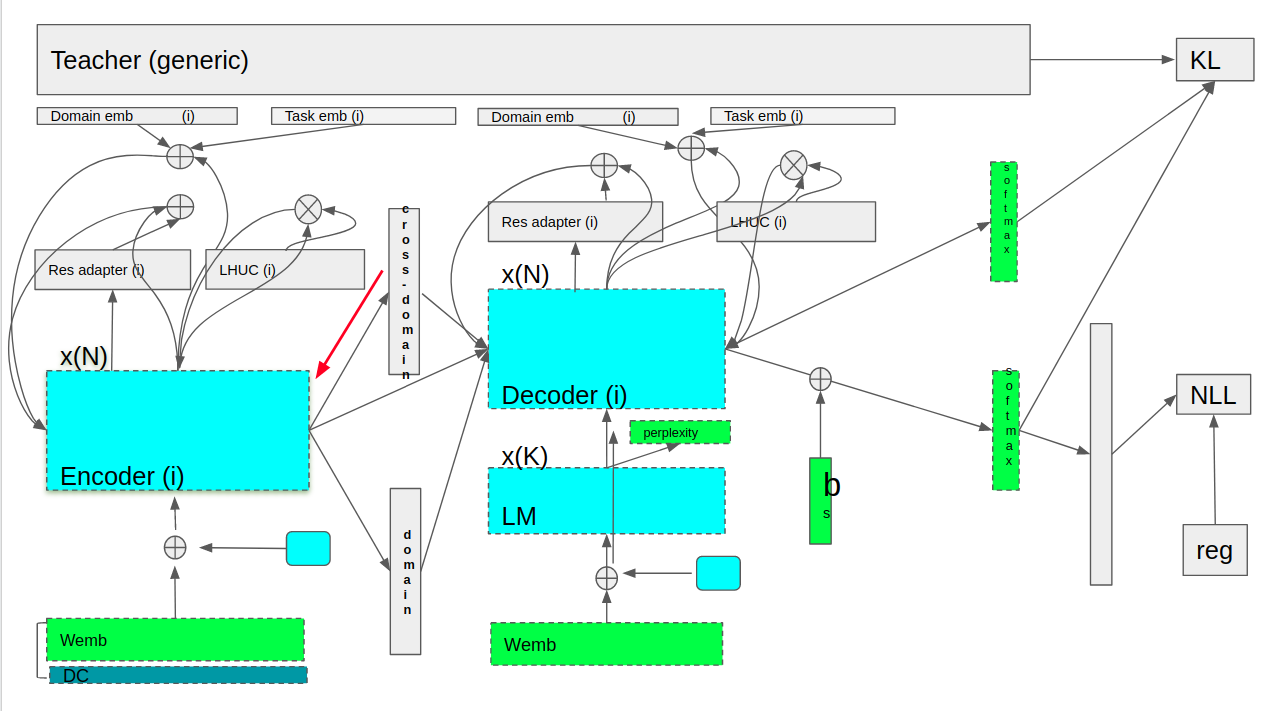
\includegraphics[scale=0.3]{DA_overview.png}
\caption{Domain Adaptation MT's overview}
\label{fig:overview}
\end{figure}

\subsection*{Realized work}
The work of \cite{Kobus17domain} and \cite{Daume07frustratingly} showed promising results for learning in a multi-domain context. Inspired by the simplicity of the methods, we extend their works to a new version of domain embedding. In this method, each word has its domain embedding which amounts to a small share of the word embedding. 


Multi-domain learning can be considered as a multi-task problem in which prediction on each domain is a task. \cite{Caruana97multitask} suggested that multi-task training can help to obtain a better generalization of a learner. A multi-task learner consists of one or stack of multiple shared lower layers and task-related modules above these later layers. By optimizing k objective functions at once, the shared layers are pulled to a compromising region between task-optimal regions. However, multi-task training has to overcome several problems such as the heterogeneity of data size, convergence rates, etc. We investigated a multi-task system based on a Transformer architecture \cite{Vaswani17attention} in a large scale multi-domain context. We reported promising results and proposed another version more adaptive. 


Many methods have been proposed to deal with multi-domain contexts but they were mostly evaluated in a very simple context which is not realistic. We took interest in designing new evaluation setups that access several desirable properties of a multi-domain system. We revisited the work of \cite{Britz17effective} \cite{Zheng18multi} \cite{Kobus17domain} and \cite{bapna19simple} in a large scale context in which there are 6-7 domains.

\section*{Lexicalized Domain Representation}
\cite{Kobus17domain} proposed to stack a domain-feature embedding to each word embedding whenever the domain appears. This way, the model pays attention to the domain from which each sample originates. However, words do not equally require domain adaptation because some of them are domain-invariant such as the articles. This property can
be handled by equipping each word its domain feature, and because these additional features are small (4 or 8 units), the method is still cheap.
\begin{figure}[h!]
  \center
  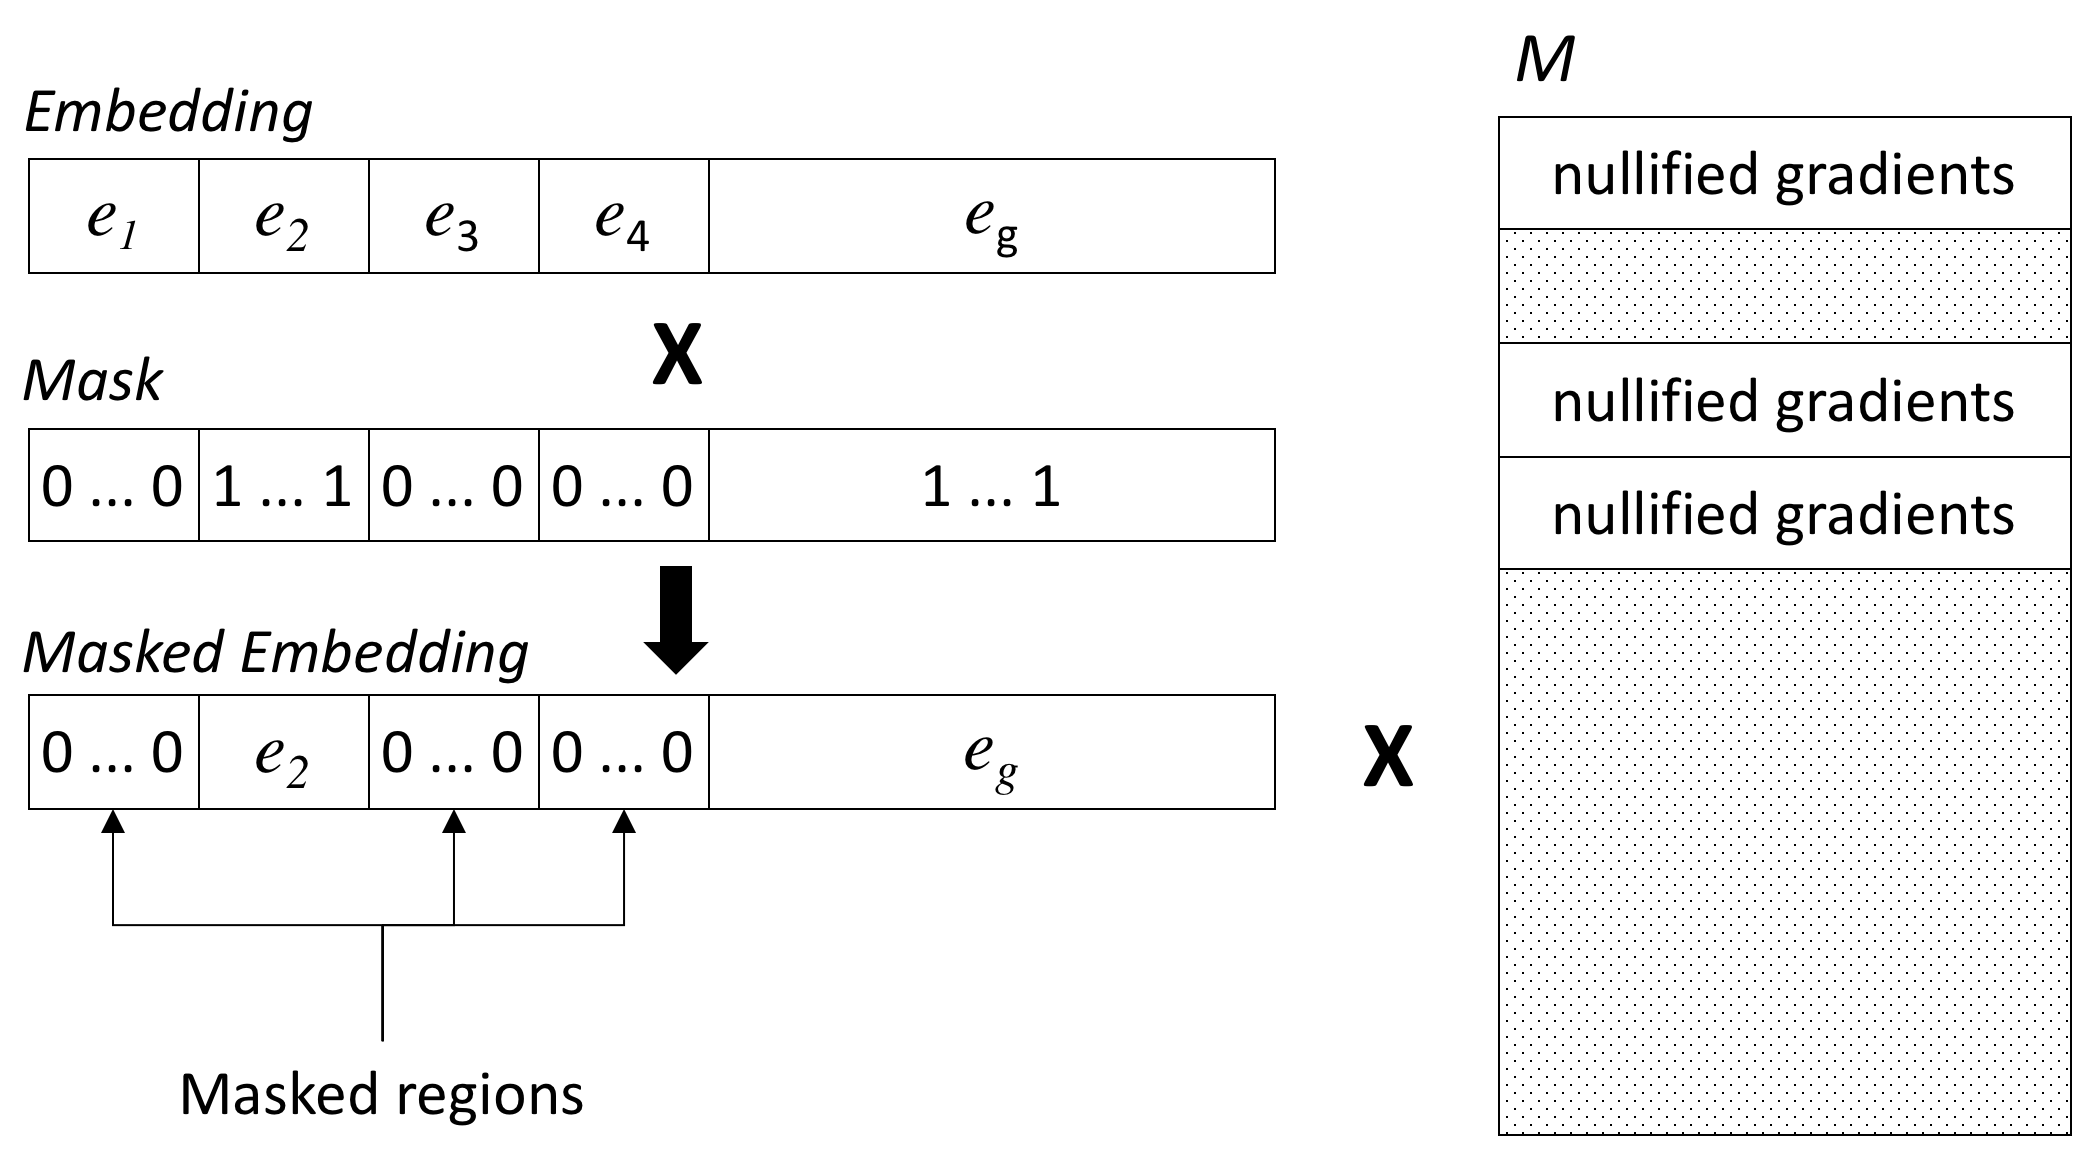
\includegraphics[width=0.48\textwidth]{embeddings}
  \caption{Lexicalized domain embeddings. When processing a sample from domain $2$, we only activate the corresponding parameter region ($\theta_2$) in the input embeddings; the remaining domain-specific parts are zeroed out and do not receive any update. The generic part is always active and is updated irrespective of the input domain.} 
  \label{fig:network}
\end{figure}

To evaluate the performance of the proposed lexicalized domain representation, experiments were performed on 2 language pairs: English $\rightarrow$ French and English $\rightarrow$ German with 3 corpora: EMEA, Europarl and ECB. The statistics of the corpora are shown in the table \ref{tab:Corpora3}
\begin{table}[h!]
  \centering
  \begin{tabular}{ |llll|} %*{4}{|r|}}
    \hline
    Corpus & Train & Valid & Test \\ 
    \hline
    \multicolumn{4}{l}{English $\rightarrow$ French }\\
    %\multicolumn{4}{|l|}{Vocab size - En: 30,165, Fr: 30,398}\\
    \hline
    EMEA  & 1.09M & 1,000 & 1,000$_{(300)}$\\
    ECB    & 0.19M & 1,000 & 1,000     \\
    EPPS   & 2.01M  & 1,000 & 1,000  \\
    IT         & 0.54M  & 1,000 & 1,000 \\  
    \hline
    \multicolumn{4}{l}{English $\rightarrow$ German}\\
    %\multicolumn{4}{|l|}{Vocab size -  En:30,159, De: 30,698}\\ 
    \hline
    EMEA  & 1.11M & 1,000 & 1,000$_{(300)}$ \\
    ECB     &  0.11M & 1,000 & 1,000  \\
    EPPS   & 1.92M & 1,000 & 1,000 \\ 
    \hline
\end{tabular}
\caption{Corpora statistics.}
\label{tab:Corpora3}
\end{table}
\begin{table}[h!]
\parbox{.42\linewidth}{
\begin{center}
\scalebox{1.0}{
\begin{tabular}{|l|lcc|c|}
\hline
Model & EMEA & EPPS & ECB & Avg. \\
\hline
%\multicolumn{8}{l}{} \\[-9pt]  
\multicolumn{5}{l}{English$\rightarrow$French} \\
\hline
$\mathtt{Mixed}$          & 67.69$_{47.60}$ & 37.50 & 53.49 & 52.89\\
\hline
$\mathtt{FT}_{EMEA}$ & 76.77$_{49.43}$ & 17.16 & 11.99 & 35.30\\
$\mathtt{FT}_{EPPS}$  & 20.86 & 37.04 & 24.53 & 27.47\\
$\mathtt{FT}_{ECB}$    & 26.93 & 27.09 & \bf 56.52 & 36.84\\
\hline
$\mathtt{DC}$              & 67.87$_{45.42}$ & 37.31 & 54.14 & 53.10\\
\hline
$\mathtt{LDR}_{oracle}$            & 74.26$_{\bf 49.90}$ & 37.67 & 54.07 & 55.33\\
$\mathtt{LDR}_{oracle}^{0.5}$   & \bf 74.95$_{49.38}$ & 37.35 & 55.91 & \bf 56.07\\
%$\mathtt{LDR}_{generic}$          & 73.97$_{49.54}$ & 37.81 & 53.67 & \\
$\mathtt{LDR}_{pred}$               & 74.29$_{49.84}$ & \bf 37.73 & 54.01 & 55.34\\
$\mathtt{LDR}_{wrong}$            & 72.95$_{49.78}$ & 37.62 & 53.35 & 54.64\\
  \hline
%\multicolumn{8}{l}{} \\[-9pt]
\multicolumn{5}{l}{English$\rightarrow$German} \\
\hline
$\mathtt{Mixed}$         & 64.57$_{42.99}$ & 26.47 & 68.67 & 53.23\\
\hline
$\mathtt{FT}_{EMEA}$ & 68.35$_{42.97}$ & 17.02 & 32.87 & 39.41\\
$\mathtt{FT}_{EPPS}$  & 36.19 & 26.29 & 40.71 & 34.39\\
$\mathtt{FT}_{ECB}$   & 24.72 & 18.36 & \bf 74.05 & 39.04\\
\hline
$\mathtt{DC}$ & 63.48$_{42.98}$ & 26.27 & 66.95 & 52.23\\
\hline
$\mathtt{LDR}_{oracle}$ & 70.90$_{\bf 46.12}$ & 26.30 & 68.90 & 55.36\\
$\mathtt{LDR}_{oracle}^{0.5}$ & \bf 71.31$_{45.23}$ & 25.98 & 73.74 & \bf 57.01\\
%$\mathtt{LDR}_{generic}$ & 70.86$_{45.60}$ & 26.14 & 68.59 & \\
$\mathtt{LDR}_{pred}$ & 70.89$_{\bf 46.12}$ & \bf 26.53 & 68.63 & 55.35\\
$\mathtt{LDR}_{wrong}$ & 69.51$_{43.50}$ & 26.31 & 66.86 & 54.22\\
\hline
\end{tabular}
} %scalebox
\end{center}
\caption{BLEU scores for  Transformer systems \label{tab:results-trsf}}
}
\hfill
\parbox{.42\linewidth}{
\begin{center}
\scalebox{1.0}{
\begin{tabular}{|l|lcc|c|}
\hline
Model & EMEA & EPPS & ECB & Avg. \\
\hline
%\multicolumn{8}{l}{} \\[-9pt]
\multicolumn{5}{l}{English$\rightarrow$French} \\
\hline
$Mixed$                         & 65.42$_{45.11}$ & 34.70 & 51.38 & 50.50\\
\hline
$\mathtt{FT}_{EMEA}$   & 72.06$_{\bf 47.33}$ & 18.62 & 16.78 & 35.82\\
$\mathtt{FT}_{EPPS}$    & 35.47$ $ & 34.61 & 39.56 & 36.55\\
$\mathtt{FT}_{ECB}$      & 21.93$ $ & 22.60 & 51.53 & 32.02\\
\hline
$\mathtt{DC}$                            & 68.26$_{43.76}$ & 35.13 & 50.09 & 51.16\\
% \hline
%$\mathtt{WDCMT}$           & 68.76$_{45.29}$ & 35.71 & 52.75 & \\
\hline
$\mathtt{LDR}_{oracle}$            & 71.73$_{46.30}$ & \bf 35.21 & 50.91 & 52.62\\
%$\mathtt{LDR_{condgru}}_{pred}$   & 71.7$_{46.21}$ & 35.09 & 51.22 & \\
$\mathtt{LDR}_{oracle}^{0.5}$   & 71.70$_{46.41}$ & 34.24& \bf 52.37 & \bf 52.77\\
%$\mathtt{LDR}_{generic}$          & 70.59$_{46.37}$ & 35.22 & 49.68 & \\
$\mathtt{LDR}_{pred}$               &\bf 72.76$_{46.35}$ & 35.10 & 50.38 & 52.75\\
$\mathtt{LDR}_{wrong}$            & 62.10$_{43.29}$ & 34.17 & 48.79 & 48.35\\
\hline
%\multicolumn{8}{l}{} \\[-9pt]
\multicolumn{5}{l}{English$\rightarrow$German} \\
\hline
$Mixed$                        & 57.37$_{37.94}$ & 23.10 & 63.54 & 48.00\\
\hline
$\mathtt{FT}_{EMEA}$  & 65.64$_{\bf 44.71}$ & 12.36 & 15.93 & 31.31\\
$\mathtt{FT}_{EPPS}$   & 24.90$ $ & 22.98 & 26.26 & 24.71\\
$\mathtt{FT}_{ECB}$     & 41.80$ $ & 15.97 & 71.07 & 42.95\\
\hline
$\mathtt{DC}$                & 62.53$_{39.25}$ & \bf 23.74 & 65.71 & 50.66\\
%\hline
%$\mathtt{WDCMT}$ & 64.05$_{38.54}$ & 22.82 & 67.00 & \\
\hline
$\mathtt{LDR}_{oracle}$     & \bf 63.43$_{40.04}$ & 22.66 & 64.40 & 50.16\\
$\mathtt{LDR}_{oracle}^{0.5}$   & 63.27$_{38.16}$ & 21.83 & \bf 69.55 & \bf 51.55\\
%$\mathtt{LDR}_{generic}$   & 63.27 $_{39.75}$ & 22.62 & 63.70 & \\
$\mathtt{LDR}_{pred}$        & 63.17$_{39.92}$ & 22.51 & 64.00 & 49.89\\
$\mathtt{LDR}_{wrong}$     & 56.84$_{37.05}$ & 22.06 & 61.66 & 46.85\\
\hline
\end{tabular}
} %scalebox
\end{center}
\caption{BLEU scores for RNN systems\label{tab:results-rnn}}
}
\end{table}
\begin{table}[!h]
\begin{center}
\scalebox{1.0}{
\begin{tabular}{|l|ccc|c|}
\hline
Model & EMEA & EPPS & ECB & Avg. \\
\hline
%\multicolumn{8}{l}{} \\[-9pt]
\multicolumn{5}{l}{English$\rightarrow$French} \\
\hline
$\mathtt{LDR}_{pred}$                   & \bf 72.76$_{46.35}$ & 35.10 & 50.38 & \bf 52.75\\
$\mathtt{LDR}_{pred}^{condgru}$  & 71.70$_{46.21}$ & 35.09 & 51.22 & 52.67\\
$\mathtt{WDCMT}$                        & 68.76$_{45.29}$ & \bf 35.71 & \bf 52.75 & 52.40\\
\hline
\end{tabular}
} %scalebox
\end{center}
\caption{BLEU scores for RNN systems. Comparison between \texttt{WDCMT} and $\texttt{LDR}_{pred}$ built using conditional GRUs.\label{tab:results-rnn-wdcmt}}
\end{table}

The baseline models consist of standard NMT model (RNN or Transformer) trained with mixing of 3 corpora; and in-domain fine-tuned models; and the last is the method proposed by \cite{Zheng18multi}. In the Transformer setting, LDR improves by a large margin the performance on domain medical and achieves on-par performance compared to the WDCNMT of \cite{Zheng18multi} on RNN architecture. More detailed results have been published in \cite{Pham19generic}.

\section*{Revisiting multi-domain NMT}
Even though many methods are proposed to solve the multi-domain problem, they were not fully evaluated. We introduced several new objectives that the multi-domain NMT system is supposed to achieve. The following are basic properties we want an NMT model to have.
\begin{enumerate}
	\item \label{ax:1} Robustness to unbalancing data.
	\item \label{ax:2} Ability to learning from other domains to improve one domain.
	\item \label{ax:3} Robustness to new domain.
	\item \label{ax:4} Ability to handle unlabeled training data (eg via clustering).
	\item \label{ax:5} Ability to perform continuous learning.
\end{enumerate}

The first property is basic because, in the real context, in-domain corpora often have a very variable size. Indeed, among OPUS corpora, the religion domain with only 130K parallel sentences (Tanzil) is very small compared to the medical domain with more than 2.5M parallel sentences (UFAL). In general, the practice of mixing corpora to train NMT down-samples the small corpora and results in low performance for these domains. 

The second is the essence of multi-domain NMT: that each domain in the mixture can benefit to the data from the other domains. 

The third property is needed to deal with unknown domains in the test phase. This situation is very common in real contexts where test data can originate from any domains. 

The fourth property is needed to deal with training data without domain information. For example, a corpus such as Paracrawl does not contain any specific topic or domain information. 

The last property is also an important and active trend in machine learning. The model needs to preserve the learned knowledge while learning as being exposed to new data.

We use the following 5 setups in our study:
\begin{enumerate}
	\item \label{setup:1} Variable-size in-domain corpora in training sets.
	\item \label{setup:2} In-domain and Out-domain test sets.
	\item \label{setup:3} Fuzzy domain separation.
	\item \label{setup:4} Training in considering unsupervised clusters as domains.
	\item \label{setup:5} Continuation of training with new domain data.
\end{enumerate}

According to our study on the state of the art of Multi-domain NMT, this is the first large scale experiment. We experimented with translation from English into French and use texts initially originating from 6 domains, corresponding to the following data sources: the UFAL Medical corpus V1.0 (\domain{med})\footnote{\url{https://ufal.mff.cuni.cz/ufal_medical_corpus}}, the European Central Bank corpus (\domain{bank}) \cite{Tiedemann12parallel}; The JRC-Acquis Communautaire corpus (\domain{law}) \cite{Steinberger06acquis}, documentations for KDE, Ubuntu, GNOME and PHP from Opus collection \cite{Tiedemann09news}, collectively merged in an \domain{it}-domain, Ted Talks (\domain{talk}) \cite{Cettolo12wit}, and the Koran (\domain{rel}). Complementary experiments \ref{setup:2} and \ref{ax:5}  also use v12 of the News Commentary corpus (\domain{news}). Corpus statistics in Table~\ref{tab:Corpora7}. Most corpora are available from the Opus web site. \footnote{\url{http://opus.nlpl.eu}}. The heterogeneity of the domain’s population is assured by the choice of in-domain corpora, therefore the property \ref{ax:1} is evaluated. (see table \ref{tab:Corpora7})

\begin{table*}[htbp]
  \centering
  \begin{tabular}{ |lllllll|} %*{4}{|r|}}
    \hline
    %\multicolumn{4}{|l|}{Vocab size - En: 30,165, Fr: 30,398}\\
    \domain{med} & \domain{law} & \domain{bank} & \domain{it} & \domain{talk} & \domain{rel} & \domain{news} \\
    \hline
    2609 (0.68) & 190 (0.05)  & 501 (0.13) & 270 (0.07) & 160 (0.04) & 130 (0.03) & 260 (0) \\
    \hline
  \end{tabular}
\caption{Corpora statistics: number of parallel lines ($\times 10^3$) and proportion in the basic domain mixture (which does not include the \domain{news} domain). \domain{med} is the largest domain, containing almost 70\% of the sentences, while \domain{rel} is the smallest, with only 3\% of the data.}
\label{tab:Corpora7}
\end{table*}

We used a test set split from the original corpus of \domain{news} to evaluate the robustness before an unknown domain. For methods requiring domain-information to predict, given a source sentence, we predict the closest domain to the sentence among already known domains.

In setup \ref{setup:3}, we randomly \emph{split} one corpus into two parts and proceed as if this corresponded to two actual domains. An MD system should detect that these two pseudo-domains are mutually beneficial, and should be hardly affected by this change with respect to the baseline scenario (no split). This setup evaluates the property \ref{ax:2}.

We also merge two corpora in training, in order to assess the robustness with respect to heterogeneous domains. We then translate the two corresponding tests with the same system. The following are 5 setups we used in the study.
\begin{itemize}
	\item Randomly splitting med data into 2 equal-sized sets.
 	\item Randomly splitting med data into 2 sets with proportions: $\frac{3}{4}$, $\frac{1}{4}$ respectively.
	\item Randomly splitting bank data into 2 equal-sized sets.
	\item Randomly splitting law data into 2 equal-sized sets.
	\item Merging bank, law into one pseudo-domain.
\end{itemize}

Setup \ref{setup:4} is used to evaluate property \ref{ax:4}. In this setup, we used k-means clustering to cluster sentence embeddings for the whole training into 30 clusters and considered them as pseudo domains. We then performed Multi-domain NMT methods with these pseudo domains. To translate a sentence, we predict the cluster which is closest to the sentence by comparing the distance between sentence embedding and the cluster means. 

The last setup \ref{setup:5} is designed to access the ability of incremental learning \ref{ax:5}. We choose \domain{news} as the 7-th domain which arrives after training with 6 domains \domain{med}, \domain{bank}, \domain{law}, \domain{rel}, \domain{talk}. We then compared the performance of the model trained by continuing training and of the model trained from scratch with 7 domains.

\section*{Multi-task network}
We can approach the multi-domain problem by multi-task learning by considering adaptation to one domain as a task. \cite{Caruana97multitask} showed multi-task training improving the performance of the model for each independent task. \cite{rebuffi18efficient} proposed the first use of a residual adapter which is a small layer plugged on top each layer to adapt classifier to an arbitrary domain. \cite{bapna19simple} reapplied the latter idea to domain adaptation in NMT. Inspired by the mentioned work in multi-task learning and domain adapter, we applied residual adapters to encoder and decoder and train the whole set of parameters from scratch. There is a small difference, instead of plugging the adapter in a sequential scheme, we propose a high-way scheme in which each adapter bridges directly from each intermediate layer to the output of the encoder. This scheme preserves the integrity of the stack of self-attention layers.

Multi-task training for K domains involves K losses on K empirical distributions. 
\begin{equation}
\begin{split}
L(\theta_{s},\theta_{i \in [1..K]}) = \frac{1}{K} \displaystyle{\mathop{\sum}_{i=[1..K]} \mathop{\sum}_{(x_i^{k},y_i^{k}) \in D_i}L(x_i^{k},y_i^{k},\theta_s,\theta_i)}
\end{split}
\label{loss:multi}
\end{equation}

We trained end-to-end the loss \ref{loss:multi}, and overcame the heterogeneity of population of the domains by using "natural" batch sampling frequency. More precisely, for each batch of stochastic training, we sample B examples from an in-domain corpus, the frequency of being picked of each corpus is proportional to the size of the corpus.
$$freq_i = \frac{\#D_i}{\displaystyle{\mathop{\sum}_{j=[1..K]}\#D_j}}$$
To avoid over-fitting for the low resource domain, we used layer activation regularization, i.e, the actual training loss is 
\begin{equation}
\begin{split}
\bar{L}(\theta_{s},\theta_{i \in [1..K]}) = L(\theta_{s},\theta_{i \in [1..K]}) + \displaystyle{\mathop{\sum}_{i \in [1..K]} \mathop{\sum}_{j \in [1..6]} \lambda_i * \normL{Adap^{j}_i(h_j)}}
\end{split}
\label{loss:multi-reg}
\end{equation}
where $\lambda_i$ is regularization scale for the adapter of domain i, $Adapt^j_i$ is the adapter for layer j in domain i. We could also adjust the capacity of each adapter to match the size of the domain training data. The adapter is composed of 5 layers:
$$Adapt(h_i) = W^{d_{model}}_{d_{Bottleneck}} * (RELU( Layernorm ( W^{d_{Bottleneck}}_{d_{model}} * Layernorm(h_i) + b_{d_{Bottleneck}} ) )) + b_{d_{model}}$$
We chosen $d_{Bottleneck}$ by grid search on set of values $\{128, 256,512,1024\}$ and $\lambda_i$ in by grid search on set of values $\times^{K}[1\minus{3}, 1\minus{4},1\minus{5},1\minus{6}]$. Optimal values of $\lambda$ could be heuristically localized by using the rule of thumb: bigger domains should yield larger $\lambda$.
\begin{figure}[h!]
\parbox{.45\linewidth}{
\begin{center}
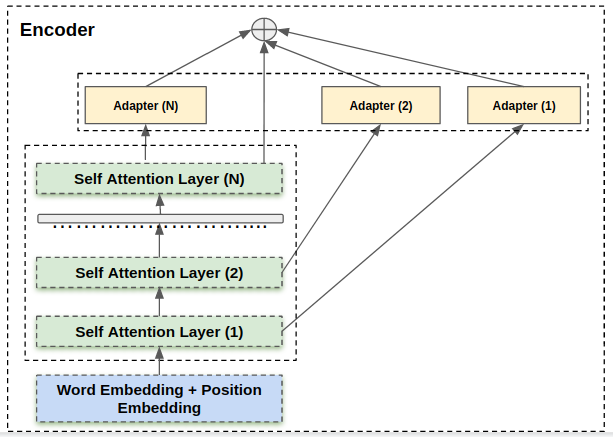
\includegraphics[scale=0.45]{highway_residual}
\caption{Highway residual adapter}
\label{fig:highwayres}
\end{center}
}
\hfill
\parbox{.45\linewidth}{
\begin{center}
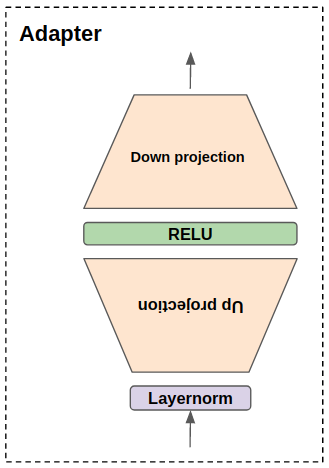
\includegraphics[scale=0.45]{adapter}
\caption{Adapter}
\label{fig:adapter}
\end{center}}
\end{figure}

\section*{Future work}
\subsection*{Adaptive Domain Adaptation}
Generalization is a basic requirement of any learner, even when in-domain data is available. NMT system often loses performance dramatically in the previous training domain after being fine-tuned to the target domain. The phenomenon is well known under the name of catastrophic forgetting which was first reported in \cite{Michael89catastrophic}. This phenomenon appears mostly in neural network systems. The reason does not until now have a well-structured answer because of the low interpretability of this architecture. In the case of machine translation, we would like to improve the generalization of the expert
system by enhancing the stability of the intermediate representation (inside the network) of word whose meaning does not change across domain while maintaining a high degree of freedom for in-domain specific words. The practice of multi-task training might have
this effect because the lower stack of encoding modules shared across tasks is pushed to stay in a region thereby realizing a trade-off between in-domain optimal regions. Words frequently shared between domains, i.e popular in most of the domains will probably fall in
this ”average” region, therefore they will have low variance with respect to domain. We would like to reinforce this behavior of the multi-domain system 

\subsection*{Multi-source adaptation}
The second problem of our interest is robustness with respect to out-of-domain data. Given several in-domain datasets in training, \cite{hoffman18algorithms}, and a test set from an unknown domain, we would like to build a good predictor from several out-of-domain expert predictors. In the machine-learning literature, the problem can be referred to as Multi-source Domain Adaptation. \cite{yishay09multiple}, \cite{mansour09domain} studied effective methods to combine learned predictors to predict test examples that come from an arbitrary unknown domain. They proposed a convex combination of learned in-domain predictors whose weights are computed by the in-domain probabilistic model. The authors also provided the upper bound of the risk of the new predictors on an arbitrary test domain. If the test distribution is not too far from the sets of a convex combination of k source distributions (in terms of Rényi divergence), then the risk of the proposed predictor on the test domain is close to the risk of the in-domain predictor on in-domain distribution. We would like to study these ideas and adapt them to our practical settings for robust multi-domain systems.

\subsection*{BPE-vocabulary's transfer effect}
One way to increase the sharing of knowledge between domains is to increase the shared vocabulary between them. By the fact that words share prefixes, suffixes between them, using smaller sequence units than words might help transfer translation information from more confident translation in high resource domain to less confident translation in low resource domains. Until now, there is not any investigation on the effect of BPE in transfer learning between domain. Therefore, we find that it is pertinent to evaluate the effect.

\section*{Other research}
\subsection*{Semantic similarity}
\cite{pham18fixing} proposed a method to predict the semantic similarity between 2 sentences from 2 different languages. The method is used in the context of filtering noisy parallel corpora such as Paracrawl. The method was implemented for corpus filtering shared task  \cite{koehn18findings}. \cite{pham18fixing} used a siamese network to encode a bilingual pair of sentences whose embedding is used to compute the semantic similarity by cosine similarity. The training of the network is done by optimizing the aggregation of soft word alignment scores between 2 sentences. To avoid being over-fitted by positive examples in which every sentence pair is correctly matched, we proposed to use the same amount of artificial negative examples in which words are randomly removed or added and changed in several positions.
\section*{Provisional planning}
\begin{itemize}
	\item Completing work on residual adapters and submission to WMT 2020 at the end of July 2020.
	\item Completing system submission to Machine Translation Robustness task of WMT 2020 at the end of July 2020.
	\item Completing work on contextualized Machine Translation with Systran's team at the end of July 2020.
	\item Completing work on Multi-source Adaptation between August - December 2020
	\item Completing work on BPE-vocabulary's transfer learning effect between January and April 2021.
\end{itemize}
\bibliography{bibliography}
\bibliographystyle{apa-good}
\end{document}


